\documentclass[paper=letter, fontsize=12pt]{article}
\usepackage{geometry}
\geometry{margin=1in}
\usepackage{graphicx}
\graphicspath{{images/}}
\usepackage{amssymb}
\usepackage{enumitem}
\usepackage{multirow}
\usepackage{longtable}

%opening
\title{Compsci 571 HW2}
\author{Yilin Gao (yg95)}

\begin{document}

\maketitle
\section{Classifier for Basketball Courts}

\begin{enumerate}[label=(\alph*)]
	% 1a
	\item When running Perceptron algorithm on the dataset, it takes 7 iterations (updates) to converge. The decision boundary is $f(x_1, x_2) = -1.05 * x_1 + 1.1 * x_2$. Because after it converges, all training points are correctly classified, the error rate is 0.
	
	Assume another linear classifier that goes through origin and achieves the same training error rate (0) as the perceptron classifier is $f(x_1, x_2) = w_1 * x_1 + w_2 * x_2$. Set $f(x_1, x_2) = 0$, we get the slope of the boundary is $-\frac{w_1}{w_2}$. From the plot of training data, we know that the boundary should go above point $[0.85, 0.80]$, and go below point $[0.85, 0.95]$. So $\frac{0.80}{0.85} < -\frac{w_1}{w_2} < \frac{0.95}{0.85}$. If we set $w_2 = 1.1$ as the perceptron boundary, we get $-1.229 < w_1 < -1.035$.
	
	The plot of observed data, the perceptron decision boundary (the light blue line), and all other linear boundaries that achieve the same training error (the yellow area) is:
	
	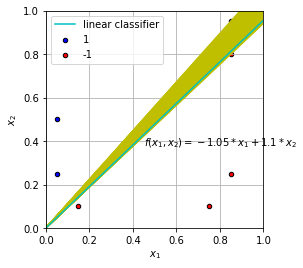
\includegraphics[scale=0.6]{q1a.png}
	
	%1b
	\item The fully-grown decision tree using Gini index as splitting criterion on the observed data is:
	
	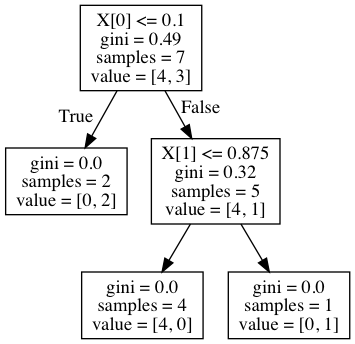
\includegraphics[scale=0.5]{q1b_tree.png}
	
	Because all training points are correctly classified by this tree, its training error is 0.
	
	Assume another decision tree with same training error (0) splits on the same feature order but different splitting threshold ($v_1$ for $x_1$ and $v_2$ for $x_2$). Then the threshold of the first split on $x_1$ should be able to separate points $[0.05, 0.25], [0.05, 0.5]$ (+1) with $[0.15, 0.1]$ (-1). So $v_1$ should be $\in (0.05, 0.15)$. The threshold of the second split on $x_2$ should be able to separate points $[0.85, 0.8]$ (-1) with $[0.85, 0.95]$ (+1). So $v_2$ should be $\in (0.8, 0.95)$.
	
	The plot of observed data, and the calculated decision boundary is:
	
	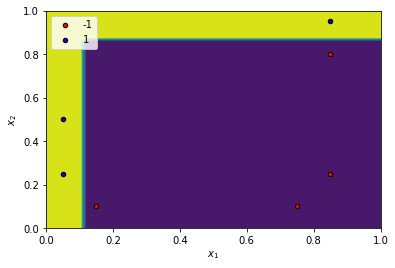
\includegraphics[scale=0.6]{q1b1.png}
	
	The plot of observed data, the calculated decision boundary, and all other decision boundaries that achieve the same training area (the red area) is:
	
	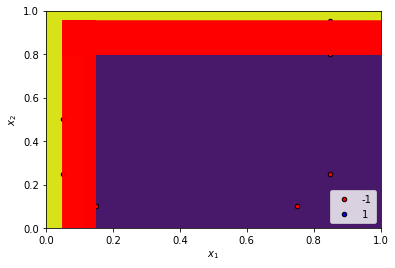
\includegraphics[scale=0.6]{q1b2.png}
	
	%1c
	\item 	Suppose the real optimal linear classifier that passes through the origin is $f(x_1, x_2) = w_1 * x_1 + w_2 * x_2$, such that it is able to minimize $R^{true}(f)$.
	
	\begin{equation}
	T = R^{true}(f) = \mathbb{E}_{(\mathbf{x}, y) \sim D}l(f(\mathbf{x}), y) = \mathbb{E}_{(\mathbf{x}, y) \sim D} \mathbf{1}_{[sign(f(\mathbf{x})) \neq y]}
	\end{equation}
	\begin{equation}
	= \mathbf{P}(sign(f(\mathbf{x})) \neq y)
	\end{equation}
	\begin{equation}
	= \mathbf{P}(y = 1, f(\mathbf{x}) \leq 0) + \mathbf{P}(y = -1, f(\mathbf{x}) \geq 0)
	\end{equation}
	\begin{equation}
	= \mathbf{P}(y = 1) * \mathbf{P}(f(\mathbf{x}) \leq 0 | y = 1) + \mathbf{P}(y = -1) * \mathbf{P}(f(\mathbf{x}) \geq 0 | y = -1)
	\end{equation}
	\begin{equation}
	= (1 - \frac{\pi}{4}) * \mathbf{P}(w_1 * x_1 + w_2 * x_2 \leq 0 | 0 \leq x_1 \leq 1, \sqrt{x_1} \leq x_2 \leq 1) 
		+ \frac{\pi}{4} * \mathbf{P}(w_1 * x_1 + w_2 * x_2 \geq 0 | 0 \leq x_1 \leq 1, 0 \leq x_2 \leq \sqrt{x_1})
	\end{equation}
	\begin{equation}
	= (1 - \frac{\pi}{4}) * \mathbf{P}(x_2 \leq -\frac{w_1}{w_2} x_1 | 0 \leq x_1 \leq 1, \sqrt{x_1} \leq x_2 \leq 1) 
	+ \frac{\pi}{4} * \mathbf{P}(x_2 \geq -\frac{w_1}{w_2} x_1 | 0 \leq x_1 \leq 1, 0 \leq x_2 \leq \sqrt{x_1})
	\end{equation}
	
	Step (2) is from the property of expectation on indicator function. Step (4) is from the rule of conditional probability. In step (5), $\mathbf{P}(y = 1) = \frac{\pi}{4}$ and $\mathbf{P}(y = -1) = 1- \frac{\pi}{4}$ because of the uniform distribution of $(x_1, x_2)$.
	
	Assign $p = -\frac{w_1}{w_2}$, $p \in [0, \infty)$, equation (6) becomes:
	
	\begin{equation}
	= (1 - \frac{\pi}{4}) * \mathbf{P}(x_2 \leq p x_1 | 0 \leq x_1 \leq 1, \sqrt{x_1} \leq x_2 \leq 1)
	+ \frac{\pi}{4} * \mathbf{P}(x_2 \geq p x_1 | 0 \leq x_1 \leq 1, 0 \leq x_2 \leq \sqrt{x_1}) 
	\end{equation}
	
	So we need to find the optimized $p$ that minimizes $R^{true}(f)$, or equivalently equation (7).
	
	If $p \in [0, 1]$, $T = \frac{\pi}{4} * (\frac{\pi}{4} - \frac{1}{2} * 1 * p)$, and local optimized $p' = 1$ minimizes $T' = \frac{\pi}{4}[\frac{\pi}{4} - \frac{1}{2}]$.
	
	If $p \in (1, \infty)$, based on geometry in the 2D space and integration, I get $T = \frac{1}{6} p^{-3} + (\frac{1}{2} - \frac{\pi}{8}) p^{-1} + (1 - \frac{\pi}{4})$. So local optimized $p'' = (1 - \frac{\pi}{4}) ^ {-2}$, and $T'' = \frac{1}{6}(1-\frac{\pi}{4})^6 - \frac{1}{2}(1-\frac{\pi}{4})^3 + (1-\frac{\pi}{4})$.
	
	So the global optimized $p^* = p'' = (1 - \frac{\pi}{4}) ^ {-2} \approx \mathbf{2.158655221735395}$, the optimal linear classifier that passes through the origin is $\mathbf{f(x_1, x_2) = -2.1587 * x_1 + 1 * x_2 = 0}$, and the corresponding minimal $R^{true}(f) = \frac{1}{6}(1-\frac{\pi}{4})^6 - \frac{1}{2}(1-\frac{\pi}{4})^3 + (1-\frac{\pi}{4}) \approx \mathbf{0.18146363796206844}$.
	
	This solution \textbf{is not} among the solutions that achieved the same loss (0) in part (a).
	
	The plot of the decision boundary (blue line) on the basketball court is:
	
	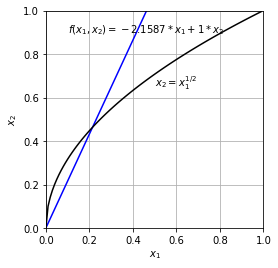
\includegraphics[scale=0.6]{q1c.png}
	
	%1d
	\item The optimal depth 2 decision tree will split on $x_1 = m$ and $x_2 = n$. And $f(\mathbf{x}) = -1$ if $m \leq x_1 \leq 1$ and $0 \leq x_2 \leq n$, $f(\mathbf{x}) = 1$ otherwise.
	
	\begin{equation}
	T = R^{true}(f) = \mathbf{P}(y = 1) * \mathbf{P}(f(\mathbf{x}) \leq 0 | y = 1) + \mathbf{P}(y = -1) * \mathbf{P}(f(\mathbf{x}) \geq 0 | y = -1)
	\end{equation}
	\begin{equation}
	= (1 - \frac{\pi}{4}) * \mathbf{P}(f(\mathbf{x}) \leq 0 | y = 1) + \frac{\pi}{4} * \mathbf{P}(f(\mathbf{x}) \geq 0 | y = -1)
	\end{equation}
	
	Step (8) comes from the same steps as in (c).
	
	If $0 \leq n \leq \sqrt{m}$, $T = \frac{\pi}{4} [1 - \frac{4}{\pi} (1-m)n] \geq \frac{\pi}{4} [1 - \frac{4}{\pi} (1-m) \sqrt{m}]$. So the local optimized $m' = \frac{1}{3}$, local optimized $n' = \sqrt{m'} = \sqrt{\frac{1}{3}}$, and local minimal $T' = \frac{\pi}{4} - \frac{2}{3}\sqrt{\frac{1}{3}} \approx 0.4004979839376978$.
	
	If $\sqrt{m} \leq n \leq 1$, according to geometry in 2D space and integration, $T = \frac{1}{3}n^3 + (\frac{\pi}{4} - 1)mn - \frac{\pi}{4}n + \frac{2}{3} m^{\frac{3}{2}} + \frac{\pi}{6}$. So the local optimized $m'' = \frac{{(4-\pi)}^2}{4^2 + 4(4-\pi) + {\pi}^2} \approx 0.025146138400079843$, local optimized $n'' = (1 - \frac{\pi}{4})m'' + \frac{\pi}{4} \approx 0.8892663104388737$, and the local minimal $T'' \approx 0.0574391669843608$.
	
	So the global optimized $m^*= \frac{{(4-\pi)}^2}{4^2 + 4(4-\pi) + {\pi}^2} \approx \mathbf{0.025146138400079843}$, the global optimized $n^* = (1 - \frac{\pi}{4})m'' + \frac{\pi}{4} \approx \mathbf{0.8892663104388737}$, and the global minimal $R^{true}(f) \approx \mathbf{0.0574391669843608}$.
	
	The real optimized tree decision boundary \textbf{is not} among those achieved in part (b).
	
	The plot of the decision boundary (blue line) on the basketball court is:
	
	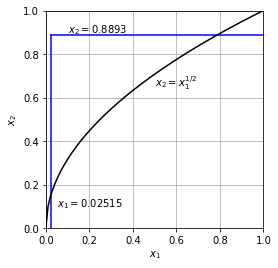
\includegraphics[scale=0.6]{q1d.png}
	
	%1e
	\item Transform $x_2$ into $\mathbf{x_2^* = x_2^2}$. So now $x_1 \in [0, 1]$, $x_2^* \in [0, 1]$, and the true boundary for the 3-point line is $x_2^* = x_1$.
	
	Suppose the real optimal linear classifier that passes through the origin is $f(x_1, x_2^*) = w_1 x_1 + w_2^* x_2^*$.
	
	\begin{equation}
	T = R^{true}(f) = \mathbf{P}(y = 1) * \mathbf{P}(f(\mathbf{x^*}) \leq 0 | y = 1) + \mathbf{P}(y = -1) * \mathbf{P}(f(\mathbf{x^*}) \geq 0 | y = -1) 
	\end{equation}
	\begin{equation}
	= \frac{1}{2} \mathbf{P}(x_2^* \leq -\frac{w_1}{w_2^*} x_1 | 0 \leq x_1 \leq 1, x_2^* \geq x_1) + \frac{1}{2} \mathbf{P}(x_2^* \geq -\frac{w_1}{w_2^*} x_1 | 0 \leq x_1 \leq 1, x_2^* \leq x_1) 
	\end{equation}
	
	And it is easy to find out that the optimal value of $\mathbf{-\frac{w_1}{w_2^*} = 1}$, the optimal linear classifier that passes through the origin is $\mathbf{f(x_1, x_2^*) = -x_1 + x_2^* = 0}$, and the corresponding minimal true error is \textbf{0}.
	
	%1f
	\item With the same transformation of $x_2$ as in part (e), suppose the optimal depth 2 decision tree splits on $x_1 = m$ and $x_2^* = n$, $R^{real}(f)$ goes as following:
	
	\begin{equation}
	T = R^{true}(f) = \mathbf{P}(y = 1) * \mathbf{P}(f(\mathbf{x^*}) \leq 0 | y = 1) + \mathbf{P}(y = -1) * \mathbf{P}(f(\mathbf{x^*}) \geq 0 | y = -1) 
	\end{equation}
	\begin{equation}
	= \frac{1}{2} * \mathbf{P}(f(\mathbf{x^*}) \leq 0 | y = 1) + \frac{1}{2} * \mathbf{P}(f(\mathbf{x^*}) \geq 0 | y = -1) 
	\end{equation}
	
	If $0 \leq n \leq m \leq 1$, $\mathbf{P}(f(\mathbf{x^*}) \leq 0 | y = 1) = 0$, $T = \frac{1}{2} [\frac{1}{2} - n(1-m)] \geq \frac{1}{2}[1-m(1-m)]$. So the local optimal $m' = \frac{1}{2}$, the local optimal $n' = \frac{1}{2}$, and the corresponding local minimal $T' = \frac{1}{8}$.
	
	If $0 \leq m < n \leq 1$, $\mathbf{P}(f(\mathbf{x^*}) \leq 0 | y = 1) = \frac{1}{2} {(n - m)}^2$, $\mathbf{P}(f(\mathbf{x^*}) \geq 0 | y = -1) = \frac{1}{2} m^2 + \frac{1}{2} {(1-n)}^2$, $T = \frac{1}{4}[{(n-m)}^2 + m^2 + {(1-n)}^2]$. The local optimized $m' = \frac{1}{3}$, $n' = \frac{2}{3}$, and the corresponding $T' = \frac{5}{24}$.
	
	So the global minimal true risk generated by a depth 2 decision tree under this transformation is $\frac{1}{8}$. The decision tree \textbf{cannot} achieve the same minimal true error (0) as the linear classifier in part (e).
	
	%1g
	\item For paint, assume the part inside paint ($0.5 \leq x_1 \leq 1$ and $0 \leq x_2 \leq 0.25$) has label $y = -1$ and the part outside paint has $y = 1$.
	 
	Same as in part (c), suppose the real optimal linear classifier that passes through the origin is $f(x_1, x_2) = w_1 * x_1 + w_2 * x_2$, such that it is able to minimize $R^{true}(f)$.
	
	\begin{equation}
	T = R^{true}(f) = \mathbf{P}(y = 1) * \mathbf{P}(f(\mathbf{x}) \leq 0 | y = 1) + \mathbf{P}(y = -1) * \mathbf{P}(f(\mathbf{x}) \geq 0 | y = -1)
	\end{equation}
	\begin{equation}
	= \frac{7}{8} * \mathbf{P}(x_2 \leq -\frac{w_1}{w_2} x_1 | y = 1) + \frac{1}{8} * \mathbf{P}(x_2 \geq -\frac{w_1}{w_2} x_1 | y = -1)
	\end{equation}
	
	Assign $p = -\frac{w_1}{w_2}$, $p \in [0, \infty)$,
	
	\begin{equation}
	= \frac{7}{8} * \mathbf{P}(x_2 \leq p x_1 | y = 1) + \frac{1}{8} * \mathbf{P}(x_2 \geq p x_1 | y = -1)
	\end{equation}
	
	If $p \geq \frac{1}{2}$, $\mathbf{P}(x_2 \geq p x_1 | y = -1) = 0$, $T = \frac{7}{8} * \mathbf{P}(x_2 \leq p x_1 | y = 1) $.
	
	\begin{enumerate}[label=(\roman*)]
		\item If $1 \geq p \geq \frac{1}{2}$, $T = \frac{7}{8}[\frac{p}{2} - \frac{1}{8}]$, and local optimized $p' = \frac{1}{2}$ generates local minimal $p' = \frac{7}{64}$.
		
		\item If $p > 1$, $T = \frac{7}{8}[\frac{7}{8} - \frac{1}{2p}]$, and local optimized $p' = 1$ generates local minimal $p' = \frac{21}{64}$.
	\end{enumerate}

	If $\frac{1}{2} > p \geq 0$,
	
	\begin{enumerate}[label=(\roman*)]
		\item If $\frac{1}{2} > p \geq \frac{1}{4}$,  $\mathbf{P}(x_2 \geq p x_1 | y = -1) = \frac{1}{8} (\frac{1}{4p} + p - 1)$, $\mathbf{P}(x_2 \leq p x_1 | y = 1) = \frac{5p}{8} - \frac{1}{4} + \frac{1}{32p}$. $T = \frac{9p}{16} + \frac{1}{32p} - \frac{15}{64}$. So the local optimized $p' = \frac{1}{4}$ generates local minimal $T' = \frac{2}{64}$.
		
		\item If $\frac{1}{4} > p \geq 0$, $\mathbf{P}(x_2 \geq p x_1 | y = -1) = \frac{1}{4}[\frac{1}{2} - 
		\frac{3p}{2}]$, $\mathbf{P}(x_2 \leq p x_1 | y = 1) = \frac{p}{8}$, $T = \frac{4p}{64} + \frac{1}{64}$. So the local optimal $p' = 0 $ generates local minimal $T' = \frac{1}{64}$.
	\end{enumerate}

	So in conclusion, the global optimized $-\frac{w_1}{w_2} = p = \mathbf{0}$, the optimal linear classifier that passes through the origin is $\mathbf{f(x_1, x_2) = x_2 = 0}$, and the corresponding minimal true error rate $R^{true}(f) = \mathbf{\frac{1}{64}}$.
	
	%1h
	\item The optimal depth 2 decision tree will split on $x_1 = m$ and $x_2 = n$. And $f(\mathbf{x}) = -1$ if $m \leq x_1 \leq 1$ and $0 \leq x_2 \leq n$, $f(\mathbf{x}) = 1$ otherwise.
	
	\begin{equation}
	T = R^{true}(f) = \mathbf{P}(y = 1) * \mathbf{P}(f(\mathbf{x}) \leq 0 | y = 1) + \mathbf{P}(y = -1) * \mathbf{P}(f(\mathbf{x}) \geq 0 | y = -1)
	\end{equation}
	\begin{equation}
	= \frac{7}{8} * \mathbf{P}(f(\mathbf{x}) \leq 0 | y = 1) + \frac{1}{8} * \mathbf{P}(f(\mathbf{x}) \geq 0 | y = -1) \geq 0
	\end{equation}
	
	It's easy to find out that when $\mathbf{m = \frac{1}{2}}$ and $\mathbf{n = \frac{1}{4}}$, both $\mathbf{P}(f(\mathbf{x}) \leq 0 | y = 1)$ and $\mathbf{P}(f(\mathbf{x}) \geq 0 | y = -1) $ are equal to 0, and $T$ achieves its minimal value \textbf{0}.
	
\end{enumerate}

\section{Variable Importance for Trees and Random Forests}

\begin{enumerate}[label=(\alph*)]
	\item 
	\begin{enumerate}[label=(\roman*)]
		\item 
		The decision stump based on the \textbf{best split} (for each node, split on the variable with largest reduction in Gini Index) is:
		
		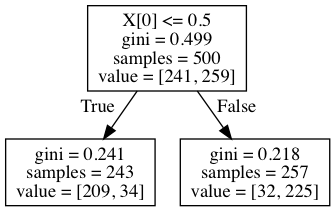
\includegraphics[scale=0.6]{tree_best_split.png}
		
		At root it splits on independent variable $X_1$ (shown as $X[0]$ in picture) on the threshold $s_1 = 0.5$.
		
		The decision stump based on the \textbf{best surrogate split} is:
		
		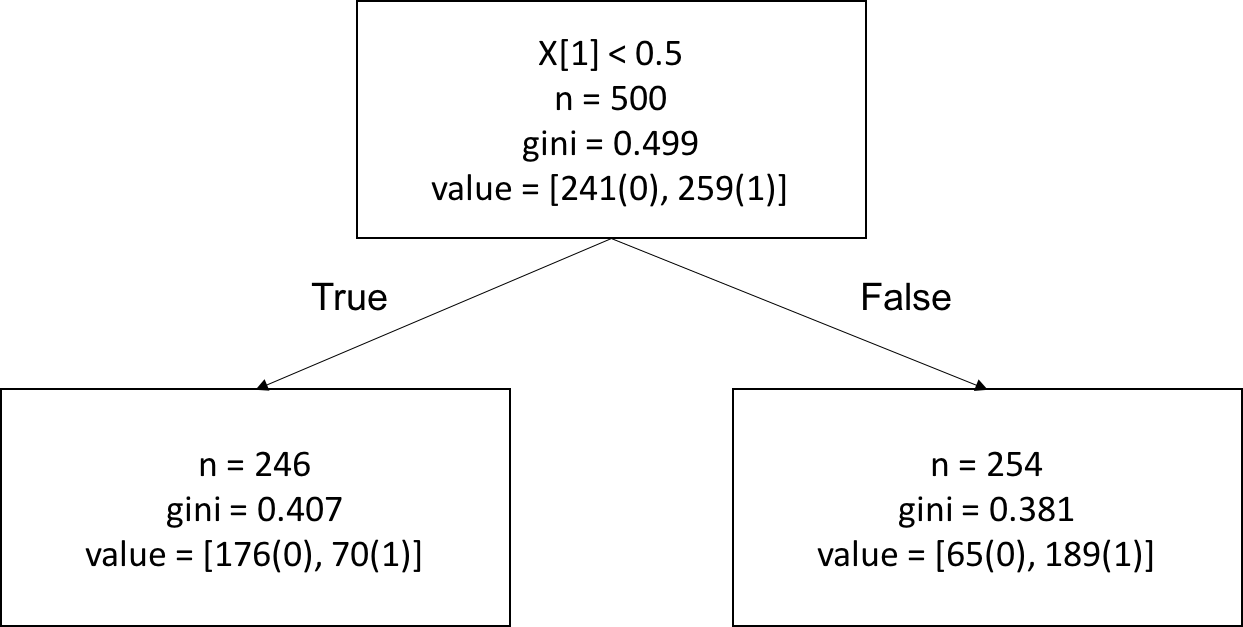
\includegraphics[scale=0.4]{tree_best_surrogate_split.png}
		
		This tree is generated by choosing the best surrogate split on the root (by comparing the predictive similarity measure on variables $X_2$, $X_3$, $X_4$ and $X_5$). At root it chooses $X_2$ (shown as $X[1]$ in picture) and threshold 0.5 (actually this value doesn't really matter) as the best surrogate split.
		
		\item Variable importance measures from equation (2) are:
		
		\begin{center}
			\begin{tabular}{|c|c|}
				\hline
				$X_1$ & $0.2706$ \\ \hline
				$X_2$ & NA \\ \hline
				$X_3$ & NA \\ \hline
				$X_4$ & NA \\ \hline
				$X_5$ & NA \\ \hline
			\end{tabular}
		\end{center}
			
		Variable importance measures from equation (3) are:
		
		\begin{center}
			\begin{tabular}{|c|c|}
				\hline
				$X_1$ & $0.2706$ \\ \hline
				$X_2$ & $0.1058$ \\ \hline
				$X_3$ & NA \\ \hline
				$X_4$ & NA \\ \hline
				$X_5$ & NA \\ \hline
			\end{tabular}
		\end{center}
	
		(See code for calculation process)
	
		If we only refer to the variable importance measures from equation (2), we can only say variable $X_1$ is the known most important variable among the five, but not sure if any other variables has similar importance as it.
		
		With the variable importance measures from equation (3), we could see comparing variable $X_1$ and its most close substitute/surrogate $X_2$, $X_1$ is still more important than $X_2$. So we could suggest with more confidence that $X_1$ is more important than others.
		
		\item 
		The mean least-squares error of predictions on the test data from the decision stump based on the best split is 0.1.
		
		The mean least-squares error of predictions on the test data from the decision stump based on the best surrogate split is 0.27. 
		
		(see code for calculation process)
		
	\end{enumerate}

	\item 
	For all following random forests, I set the seed in Python numpy to 111.
	
	\begin{enumerate}[label=(\roman*)]
		\item The table for best split variable for each $K$ is:
		
		\begin{center}
			\begin{longtable}{|c|c|c|}
				\hline
				$K$ & variable & time as best split variable (out of 1000) \\ \hline
				\multirow{5}{1em}{1} & $X_1$ & 200 \\ 
				& $X_2$ & 205 \\
				& $X_3$ & 196 \\
				& $X_4$ & 209 \\
				& $X_5$ & 190 \\
				\hline
				\multirow{5}{1em}{2} & $X_1$ & 333 \\ 
				& $X_2$ & 278 \\
				& $X_3$ & 157 \\
				& $X_4$ & 156 \\
				& $X_5$ & 76 \\
				\hline
				\multirow{5}{1em}{3} & $X_1$ & 509 \\ 
				& $X_2$ & 283 \\
				& $X_3$ & 79 \\
				& $X_4$ & 93 \\
				& $X_5$ & 36 \\
				\hline
				\multirow{5}{1em}{4} & $X_1$ & 588 \\ 
				& $X_2$ & 280 \\
				& $X_3$ & 56 \\
				& $X_4$ & 53 \\
				& $X_5$ & 23 \\
				\hline
				\multirow{5}{1em}{5} & $X_1$ & 668 \\ 
				& $X_2$ & 237 \\
				& $X_3$ & 46 \\
				& $X_4$ & 29 \\
				& $X_5$ & 20 \\
				\hline
			\end{longtable}
		\end{center}	
		
		The table for best split surrogate split variable for each $K$ is:
		
		\begin{center}
			\begin{longtable}{|c|c|c|}
				\hline
				$K$ & variable & time as best surrogate split variable (out of 1000) \\ \hline
				\multirow{5}{1em}{1} & $X_1$ & 0 \\ 
				& $X_2$ & 0 \\
				& $X_3$ & 0 \\
				& $X_4$ & 0 \\
				& $X_5$ & 0 \\
				\hline
				\multirow{5}{1em}{2} & $X_1$ & 29 \\ 
				& $X_2$ & 115 \\
				& $X_3$ & 275 \\
				& $X_4$ & 263 \\
				& $X_5$ & 318 \\
				\hline
				\multirow{5}{1em}{3} & $X_1$ & 109 \\ 
				& $X_2$ & 254 \\
				& $X_3$ & 237 \\
				& $X_4$ & 167 \\
				& $X_5$ & 233 \\
				\hline
				\multirow{5}{1em}{4} & $X_1$ & 177 \\ 
				& $X_2$ & 345 \\
				& $X_3$ & 173 \\
				& $X_4$ & 107 \\
				& $X_5$ & 198 \\
				\hline
				\multirow{5}{1em}{5} & $X_1$ & 258 \\ 
				& $X_2$ & 398 \\
				& $X_3$ & 127 \\
				& $X_4$ & 68 \\
				& $X_5$ & 149 \\
				\hline
			\end{longtable}
		\end{center}
	
		According to best split variable, $X_1$ is selected as the best split variable more as $K$ increases. So this suggests variable $X_1$ is more important than others.
		
		And according to best surrogate split variable, $X_2$ is selected more as $K$ increases. So this suggests while $X_1$ is important, the importance of $X_2$ could have been masked by that of $X_1$. So we also need to consider the importance of $X_2$.
		
		\item The variable importance according to equations (5) and (6) for each $K$ is:
		
		\begin{longtable}{|c|c|c|c|}
			\hline
			$K$ & variable & variable importance (5) & variable importance (6) \\ \hline
			\multirow{5}{1em}{1} & $X_1$ & 0.315591 & 0.365900 \\ 
			& $X_2$ & 0.184543 & 0.230439 \\
			& $X_3$ & 0.087096 & -0.017959 \\
			& $X_4$ & 0.100569 & 0.009761 \\
			& $X_5$ & 0.091519 & -0.026316 \\
			\hline
			\multirow{5}{1em}{2} & $X_1$ & 0.315598 & 0.364745 \\ 
			& $X_2$ & 0.184487 & 0.227410 \\
			& $X_3$ & 0.086678 & -0.010318 \\
			& $X_4$ & 0.100980 & -0.007949 \\
			& $X_5$ & 0.091208 & -0.022895 \\
			\hline
			\multirow{5}{1em}{3} & $X_1$ & 0.316503 & 0.367819 \\ 
			& $X_2$ & 0.184912 & 0.228975 \\
			& $X_3$ & 0.086697 & -0.010125 \\
			& $X_4$ & 0.101133 & -0.008817 \\
			& $X_5$ & 0.091880 & -0.038887 \\
			\hline
			\multirow{5}{1em}{4} & $X_1$ & 0.316615 & 0.364218 \\ 
			& $X_2$ & 0.185013 & 0.233357 \\
			& $X_3$ & 0.088056 & -0.013214 \\
			& $X_4$ & 0.100946 & -0.001885 \\
			& $X_5$ & 0.091464 & -0.031304 \\
			\hline
			\multirow{5}{1em}{5} & $X_1$ & 0.316620 & 0.363772 \\ 
			& $X_2$ & 0.185098 & 0.228608 \\
			& $X_3$ & 0.087510 & -0.013913 \\
			& $X_4$ & 0.100940 & -0.014481 \\
			& $X_5$ & 0.090950 & -0.037 \\
			\hline
		\end{longtable}
		
		%TODO masking
		
		\item The mean squares loss on the test data using the random forest with 2 methods:
		
		\begin{center}
			\begin{tabular}{|c|c|c|}
				\hline
				$K$ & method 1 & method 2 \\ \hline
				1 &  & \\ \hline
				2 &  & \\ \hline
				3 &  & \\ \hline
				4 &  & \\ \hline
				5 &  & \\ \hline
			\end{tabular}
		\end{center}
		
		%TODO which method is correct for random forest
	\end{enumerate}

	\item 
	\begin{enumerate}[label=(\roman*)]
		\item The variable importance according to equations (5) and (6) for each $q$ is:
		
		\begin{longtable}{|c|c|c|c|}
			\hline
			$q$ & variable & variable importance (5) & variable importance (6) \\ \hline
			\multirow{5}{1em}{0.4} & $X_1$ & 0.407452 & 0.367130 \\ 
			& $X_2$ & 0.341932 & 0.229640 \\
			& $X_3$ & 0.286466 & -0.015229\\
			& $X_4$ & 0.300333 & 0.001737 \\
			& $X_5$ & 0.290861 & -0.012727 \\
			\hline
			\multirow{5}{1em}{0.5} & $X_1$ & 0.383744 & 0.367407 \\ 
			& $X_2$ & 0.301408 & 0.233945 \\
			& $X_3$ & 0.236769 & -0.012283 \\
			& $X_4$ & 0.250323 & 0.003333 \\
			& $X_5$ & 0.241498 & -0.016509 \\
			\hline
			\multirow{5}{1em}{0.6} & $X_1$ & 0.361694 & 0.367335 \\ 
			& $X_2$ & 0.263844 & 0.226786 \\
			& $X_3$ & 0.187090 & -0.017031 \\
			& $X_4$ & 0.200351 & 0.002857 \\
			& $X_5$ & 0.191520 & -0.020842 \\
			\hline
			\multirow{5}{1em}{0.7} & $X_1$ & 0.339353 & 0.365197 \\ 
			& $X_2$ & 0.224097 & 0.224492 \\
			& $X_3$ & 0.137176 & -0.020660 \\
			& $X_4$ & 0.150509 & 0.003743 \\
			& $X_5$ & 0.141717 & -0.016368\\
			\hline
			\multirow{5}{1em}{0.8} & $X_1$ & 0.315598 & 0.364745 \\ 
			& $X_2$ & 0.184488 & 0.227410 \\
			& $X_3$ & 0.086678 & -0.010318 \\
			& $X_4$ & 0.100980 & -0.007947 \\
			& $X_5$ & 0.091208 & -0.022893 \\
			\hline
		\end{longtable}
		
		%TODO 
		From the results, 
		
		\item The standard deviation of variable importance according to equations (5) and (6) for each $q$ is:
		
		\begin{longtable}{|c|c|c|c|}
			\hline
			$q$ & variable & std (5) & std (6) \\ \hline
			\multirow{5}{1em}{0.4} & $X_1$ & 0.01112367 & 0.03103856 \\ 
			& $X_2$ & 0.00870762 & 0.03255196 \\
			& $X_3$ & 0.00952271 & 0.03317124 \\
			& $X_4$ & 0.00323389 & 0.04077185 \\
			& $X_5$ & 0.00681136 & 0.0327284 \\
			\hline
			\multirow{5}{1em}{0.5} & $X_1$ & 0.01124836 & 0.03793574 \\ 
			& $X_2$ & 0.00902561 & 0.03685835 \\
			& $X_3$ & 0.00797128 & 0.03568958 \\
			& $X_4$ & 0.0028276 & 0.04255715 \\
			& $X_5$ & 0.00608335 & 0.04003311 \\
			\hline
			\multirow{5}{1em}{0.6} & $X_1$ & 0.01055884 & 0.04240423 \\ 
			& $X_2$ & 0.00876408 & 0.04514072 \\
			& $X_3$ & 0.00609878 & 0.04217448 \\
			& $X_4$ & 0.00215396 & 0.0493615 \\
			& $X_5$ & 0.00455622 & 0.03715297 \\
			\hline
			\multirow{5}{1em}{0.7} & $X_1$ & 0.01003214 & 0.04752654 \\ 
			& $X_2$ & 0.00857417 & 0.04998027 \\
			& $X_3$ & 0.00480541 & 0.04686512 \\
			& $X_4$ & 0.00181428 & 0.05767446 \\
			& $X_5$ & 0.00400655 & 0.04974323 \\
			\hline
			\multirow{5}{1em}{0.8} & $X_1$ & 0.00833034 & 0.06041158 \\ 
			& $X_2$ & 0.00750252 & 0.0628672 \\
			& $X_3$ & 0.00366868 & 0.06426875 \\
			& $X_4$ & 0.00133906 & 0.06270319 \\
			& $X_5$ & 0.00315306 & 0.05855308 \\
			\hline
		\end{longtable}
	\end{enumerate}
\end{enumerate}
\end{document}
